\newpage
\section{Introducc\'ion}

Utilizando verilog, se realiza un proyecto para la entrega del trabajo final de la materia arquitectura de computadoras 2012. El proyecto consiste en la construcción de un pipeline de 5 etapas capaz de decodificar un código previamente cargado y que este sea capaz de procesarlo, llegando hasta la ejecución, por último con fines de evaluación y verficaci\'on embeber el c\'odigo desarrollado en una fpga y correr un programa desarrollado que demuestre el funcionamiento.

\subsection{IDE}
El entorno de desarrollo utilizado para el desarrollo del c\'odigo del pipeline es el \texttt{Project Navigator, release version 14.4 (lin), Aplication version:P49d}.
Para desarrolar la interfaz gr\'afica de debug se utiliz\'o el editor de interfaces \texttt{glade} y se program\'o la recepci\'on de datos en \texttt{python 2.7}. 

\subsection{SVN}
Se llev\'o a cabo el desarrallo del software utilizando un servidor svn para el control de cambios que facilit\'o la tarea a la hora de volver hacia ``c\'odigo estable'' y desde all\'i retomar el desarrollo.

\subsection{Placa de desarrollo}
Para embeber el c\'odigo se utiliz\'o la placa de desarrollo de \texttt{Digilent, Nexys™3 Spartan-6 FPGA Board} con frecuencia de 100 MHZ, las caracter\'isticas de la placa se detallan en la figura \ref{fig:digilent}.
\begin{figure}[H]
\centering
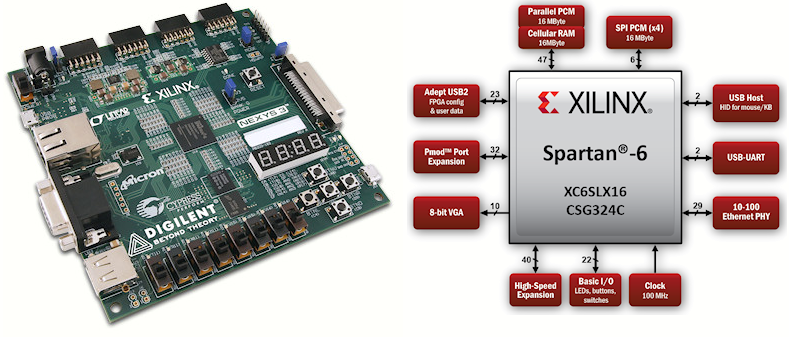
\includegraphics[scale=0.5]{img/digilent}
\caption{Placa de desarrollo}
\label{fig:digilent}
\end{figure} 		 
\newpage		

\subsection{Set de instrucciones implementado}

Para comenzar con el trabajo pr\'actico necesitamos saber cuales son las instrucciones que entran en juego en el pipeline. Una vez hecho esto podemos comenzar primero por un parser que verifique el estado de las instrucciones (si están correctamente escritas), para luego ejecutarlas con el pipeline.

\subsubsection{Instrucciones}
\textbf{Tipo I}\\

\texttt{LW (Load word)}

\begin{lstlisting}[style=consola]
32                             16                               0
+-+-+-+-+-+-+-+-+-+-+-+-+-+-+-+-+-+-+-+-+-+-+-+-+-+-+-+-+-+-+-+-+
|1 0 0 0 1 1|   base  |   rt    |              offset           |
+-+-+-+-+-+-+-+-+-+-+-+-+-+-+-+-+-+-+-+-+-+-+-+-+-+-+-+-+-+-+-+-+
+----6------+----5----+---5-----+---------------16--------------+

Formato: LW rt,offset(base)
Proposito: Guarda una palabra desde memoria a registro.
Descripcion: rt <- memory[base+offset]
\end{lstlisting}

\texttt{SW(store word)}

\begin{lstlisting}[style=consola]
32                             16                               0
+-+-+-+-+-+-+-+-+-+-+-+-+-+-+-+-+-+-+-+-+-+-+-+-+-+-+-+-+-+-+-+-+
|1 0 1 0 1 1|  base   |   rt    |             offset            |
+-+-+-+-+-+-+-+-+-+-+-+-+-+-+-+-+-+-+-+-+-+-+-+-+-+-+-+-+-+-+-+-+
+----6------+---5-----+---5-----+---------------16--------------+

Formato: SW rt,offset(base)
Proposito: Guarda palabra en memoria.
Descripcion: memory[base+offset] <- rt
\end{lstlisting}

\texttt{ADDI (Add Inmediate Word)}

\begin{lstlisting}[style=consola]
32                             16                               0
+-+-+-+-+-+-+-+-+-+-+-+-+-+-+-+-+-+-+-+-+-+-+-+-+-+-+-+-+-+-+-+-+
|0 0 1 0 0 0|   rs    |   rt    |            inmediate          |
+-+-+-+-+-+-+-+-+-+-+-+-+-+-+-+-+-+-+-+-+-+-+-+-+-+-+-+-+-+-+-+-+
+----6------+---5-----+---5-----+---------------16--------------+

Formato: ADDI rt, rs, inmediate
Proposito: Suma una constante a un entero de 32 bits. Si ocurre un overflow, then trap.
Descripcion: rt <- rs + inmediate
\end{lstlisting}

\texttt{ANDI (And Inmediate)}

\begin{lstlisting}[style=consola]
32                             16                               0
+-+-+-+-+-+-+-+-+-+-+-+-+-+-+-+-+-+-+-+-+-+-+-+-+-+-+-+-+-+-+-+-+
|0 0 1 1 0 0|   rs    |   rt    |            inmediate          |
+-+-+-+-+-+-+-+-+-+-+-+-+-+-+-+-+-+-+-+-+-+-+-+-+-+-+-+-+-+-+-+-+
+----6------+---5-----+---5-----+---------------16--------------+

Formato: ANDI rt, rs, inmediate
Proposito: Hace bit a bit la operacion logica AND con una constante.
Descripcion: rt <- rs AND immediate
\end{lstlisting}

\texttt{ORI (OR Inmediate)}

\begin{lstlisting}[style=consola]
32                             16                               0
+-+-+-+-+-+-+-+-+-+-+-+-+-+-+-+-+-+-+-+-+-+-+-+-+-+-+-+-+-+-+-+-+
|0 0 1 1 0 1|   rs    |   rt    |            inmediate          |
+-+-+-+-+-+-+-+-+-+-+-+-+-+-+-+-+-+-+-+-+-+-+-+-+-+-+-+-+-+-+-+-+
+----6------+---5-----+---5-----+---------------16--------------+

Formato: ORI rt, rs, immediate
Proposito: Hace una operacion logica OR bit a bit con una constante.
Descripcion: rd <- rs OR immediate
\end{lstlisting}

\texttt{XORI (Exclusive OR Immediate)}

\begin{lstlisting}[style=consola]
32                             16                               0
+-+-+-+-+-+-+-+-+-+-+-+-+-+-+-+-+-+-+-+-+-+-+-+-+-+-+-+-+-+-+-+-+
|0 0 1 1 1 0|   rs    |   rt    |            inmediate          |
+-+-+-+-+-+-+-+-+-+-+-+-+-+-+-+-+-+-+-+-+-+-+-+-+-+-+-+-+-+-+-+-+
+----6------+---5-----+---5-----+---------------16--------------+

Formato: XORI rt, rs, immediate
Proposito: Hace una operacion logica OR bit a bit con una constante.
Descripcion: rt <- rs XOR inmediate
\end{lstlisting}

\texttt{SLTI(Set on Less Than Inmediate)}

\begin{lstlisting}[style=consola]
32                             16                               0
+-+-+-+-+-+-+-+-+-+-+-+-+-+-+-+-+-+-+-+-+-+-+-+-+-+-+-+-+-+-+-+-+
|0 0 1 0 1 0|   rs    |   rt    |           inmediate           |
+-+-+-+-+-+-+-+-+-+-+-+-+-+-+-+-+-+-+-+-+-+-+-+-+-+-+-+-+-+-+-+-+
+----6------+---5-----+---5-----+---------------16--------------+

Formato: SLTI rt, rs, inmediate
Proposito: Guarda el resultado de la comparacion con la constante. Coloca 1 en rt si rs es menor que el inmediato.
Descripcion: rt <- (rs < inmediate)
\end{lstlisting}

\texttt{BEQ(Branch on Equal)}

\begin{lstlisting}[style=consola]
32                             16                               0
+-+-+-+-+-+-+-+-+-+-+-+-+-+-+-+-+-+-+-+-+-+-+-+-+-+-+-+-+-+-+-+-+
|0 0 0 1 0 0|   rs    |   rt    |             offset            |
+-+-+-+-+-+-+-+-+-+-+-+-+-+-+-+-+-+-+-+-+-+-+-+-+-+-+-+-+-+-+-+-+
+----6------+---5-----+---5-----+---------------16--------------+

Formato: BEQ rs, rt, offset
Proposito: Compara si son iguales y salta.
Descripcion: if (rs = rt) luego salta.
\end{lstlisting}

\texttt{BNE(Branch on Not Equal)}

\begin{lstlisting}[style=consola]
32                             16                               0
+-+-+-+-+-+-+-+-+-+-+-+-+-+-+-+-+-+-+-+-+-+-+-+-+-+-+-+-+-+-+-+-+
|0 0 0 1 0 1|   rs    |   rt    |          offset               |
+-+-+-+-+-+-+-+-+-+-+-+-+-+-+-+-+-+-+-+-+-+-+-+-+-+-+-+-+-+-+-+-+
+----6------+---5-----+---5-----+---------------16--------------+

Formato: BNE rs, rt, offset
Proposito: Compara si son distintos y salta.
Descripcion: if (rs != rt) luego salta.
\end{lstlisting}

\texttt{J(Jump)}

\begin{lstlisting}[style=consola]
32                             16                               0
+-+-+-+-+-+-+-+-+-+-+-+-+-+-+-+-+-+-+-+-+-+-+-+-+-+-+-+-+-+-+-+-+
|0 0 0 0 1 0|            instr_index                            |
+-+-+-+-+-+-+-+-+-+-+-+-+-+-+-+-+-+-+-+-+-+-+-+-+-+-+-+-+-+-+-+-+
+----6------+-----------------------26--------------------------+

Formato: J target
Proposito: Salto dentro de los siguientes 256 MB.
\end{lstlisting}

\texttt{ADD(Add Word)}

\begin{lstlisting}[style=consola]
32                             16                               0
+-+-+-+-+-+-+-+-+-+-+-+-+-+-+-+-+-+-+-+-+-+-+-+-+-+-+-+-+-+-+-+-+
|0 0 0 0 0 0|  rs     |  rt     |  rd     |0 0 0 0 0|1 0 0 0 0 0|
+-+-+-+-+-+-+-+-+-+-+-+-+-+-+-+-+-+-+-+-+-+-+-+-+-+-+-+-+-+-+-+-+
+----6------+----5----+----5----+---5-----+----5----+-----6-----+

Formato: ADD rd, rs, rt
Proposito: To add 32-bit integers. If overflow occurs, then trap.
Descripcion: rd <- rs + rt
\end{lstlisting}

\texttt{SUB(Subtract Word)}

\begin{lstlisting}[style=consola]
32                             16                               0
+-+-+-+-+-+-+-+-+-+-+-+-+-+-+-+-+-+-+-+-+-+-+-+-+-+-+-+-+-+-+-+-+
|0 0 0 0 0 0|   rs    |   rt    |   rd    |0 0 0 0 0|1 0 0 0 1 0|
+-+-+-+-+-+-+-+-+-+-+-+-+-+-+-+-+-+-+-+-+-+-+-+-+-+-+-+-+-+-+-+-+
+----6------+----5----+----5----+---5-----+----5----+-----6-----+

Formato: SUB rd, rs, rt
Proposito: Para restar enteros de 32 bits.
Descripcion: rd <- rs - rt
\end{lstlisting}

\texttt{AND (And)}

\begin{lstlisting}[style=consola]
32                             16                               0
+-+-+-+-+-+-+-+-+-+-+-+-+-+-+-+-+-+-+-+-+-+-+-+-+-+-+-+-+-+-+-+-+
|0 0 0 0 0 0|   rs    |   rt    |   rd    |0 0 0 0 0|1 0 0 1 0 0|
+-+-+-+-+-+-+-+-+-+-+-+-+-+-+-+-+-+-+-+-+-+-+-+-+-+-+-+-+-+-+-+-+
+----6------+----5----+----5----+---5-----+----5----+-----6-----+

Formato: AND rd, rs, rt
Proposito: Operacion logica AND bit a bit.
Descripcion: rd <- rs AND rt
\end{lstlisting}

\texttt{OR(or)}

\begin{lstlisting}[style=consola]
32                             16                               0
+-+-+-+-+-+-+-+-+-+-+-+-+-+-+-+-+-+-+-+-+-+-+-+-+-+-+-+-+-+-+-+-+
|0 0 0 0 0 0|   rs    |   rt    |   rd    |0 0 0 0 0|1 0 0 1 0 1|
+-+-+-+-+-+-+-+-+-+-+-+-+-+-+-+-+-+-+-+-+-+-+-+-+-+-+-+-+-+-+-+-+
+----6------+----5----+----5----+---5-----+----5----+-----6-----+

Formato: OR rd, rs, rt
Proposito: Operacion logica OR bit a bit.
Descripcion: rd <- rs OR rt
\end{lstlisting}

\texttt{XOR(Exclusive OR)}

\begin{lstlisting}[style=consola]
32                             16                               0
+-+-+-+-+-+-+-+-+-+-+-+-+-+-+-+-+-+-+-+-+-+-+-+-+-+-+-+-+-+-+-+-+
|0 0 0 0 0 0|   rs    |   rt    |   rd    |0 0 0 0 0|1 0 0 1 1 0|
+-+-+-+-+-+-+-+-+-+-+-+-+-+-+-+-+-+-+-+-+-+-+-+-+-+-+-+-+-+-+-+-+
+----6------+----5----+----5----+---5-----+----5----+-----6-----+

Formato: XOR rd, rs, rt
Proposito: Operacion logica OR EXCLUSIVA bit a bit.
Descripcion: rd <- rs XOR rt
\end{lstlisting}

\texttt{NOR(Not OR)}

\begin{lstlisting}[style=consola]
32                             16                               0
+-+-+-+-+-+-+-+-+-+-+-+-+-+-+-+-+-+-+-+-+-+-+-+-+-+-+-+-+-+-+-+-+
|0 0 0 0 0 0|   rs    |   rt    |   rd    |0 0 0 0 0|1 0 0 1 1 1|
+-+-+-+-+-+-+-+-+-+-+-+-+-+-+-+-+-+-+-+-+-+-+-+-+-+-+-+-+-+-+-+-+
+----6------+----5----+----5----+---5-----+----5----+-----6-----+

Formato: NOR rd, rs, rt
Proposito: Operacion logica bit a bit NOT OR
Descripcion: rd <- rs NOR rt
\end{lstlisting}

\texttt{SLT(Set On Less Than)}

\begin{lstlisting}[style=consola]
32                             16                               0
+-+-+-+-+-+-+-+-+-+-+-+-+-+-+-+-+-+-+-+-+-+-+-+-+-+-+-+-+-+-+-+-+
|0 0 0 0 0 0|   rs    |   rt    |   rd    |0 0 0 0 0|1 0 1 0 1 0|
+-+-+-+-+-+-+-+-+-+-+-+-+-+-+-+-+-+-+-+-+-+-+-+-+-+-+-+-+-+-+-+-+
+----6------+----5----+----5----+---5-----+----5----+-----6-----+

Formato: SLT rd, rs, rt
Proposito: Guarda el resultado de la comparacion. Coloca 1 en rt si rs es menor que el inmediato.
Descripcion: rd <- (rs < rt)
\end{lstlisting}